\section{PS3a: N-Body Simulation (Static)}\label{sec:ps3a}

\subsection{Discussion}\label{sec:ps3a:disc}

This program reads the text file which stored the informations of numbers, names, sizes, postions, and speed of planets, and takes those information in it and register them into the program and run.
This program uses SFML library, to put the planet pictures on the window.

\begin{figure}[tbh]
	\centering
	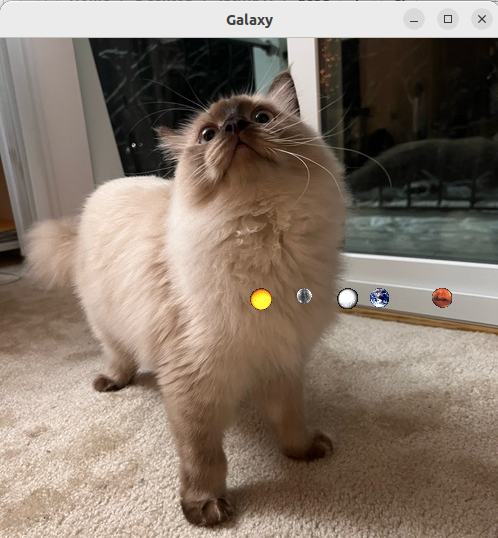
\includegraphics[width=8cm]{ps3a}
	\caption{The program shows the planets}
	\label{fig:ps3a}
\end{figure}


\subsection{Places to get help}

I got help from c++.com, stackoverflow, and Izzy from Dr.Daly's discord group.

\subsection{What I accomplished}\label{sec:ps3a:accomplish}

I used vector because I used vector for the previous program, so it was easier than other containers to declare the planets. I drew the planets with iterator since I used vector, so it was easy to draw.
.gch files get produced when I compile, but I put the code in Makefile that it cleans it. 

%\subsection{What I already knew}\label{sec:ps0:knew}

\subsection{What I learned}\label{sec:ps3a:learned}

I learned how to read the file and store it in to the class member by using these codes.
\lstinputlisting{ps3a/ps3aIn.cpp}

\subsection{Challenges}\label{sec:ps3a:challenges}
when I compile the codes, it shows error with .hpp files. It said it has problem with pragma once, but if I compile it again, it compiles fine. 
I got a feedback from my professor that I was trying to compile .hpp file.

Also, I tried to put vector variable for planets in the private member, but I could not because I did not know how to push back the vector as private member.

\subsection{Mistakes}\label{sec:ps3a:Mistakes}

I got 3 points off because yaxis is inverted, Universe not Drawable, and vector variable was in public field.

\subsection{Extra Credit}\label{sec:ps3a:Extra Credit}

I got one extra credit because I put the background picture.

\subsection{Codebase}\label{sec:ps3a:code}
Makefile
\lstinputlisting[language=Make]{ps3a/Makefile}
main.cpp
\lstinputlisting{ps3a/main.cpp}
universe.hpp
\lstinputlisting{ps3a/universe.hpp}
universe.cpp
\lstinputlisting{ps3a/universe.cpp}
CelestialBody.hpp
\lstinputlisting{ps3a/CelestialBody.hpp}
CelestialBody.cpp
\lstinputlisting{ps3a/CelestialBody.cpp}

\newpage
